% !TEX TS-program = pdflatex
% !TEX encoding = UTF-8 Unicode

% This is a simple template for a LaTeX document using the "article" class.
% See "book", "report", "letter" for other types of document.

\documentclass[11pt]{article} % use larger type; default would be 10pt

\usepackage[utf8]{inputenc} % set input encoding (not needed with XeLaTeX)

%%% Examples of Article customizations
% These packages are optional, depending whether you want the features they provide.
% See the LaTeX Companion or other references for full information.

%%% PAGE DIMENSIONS
\usepackage{geometry} % to change the page dimensions
\geometry{a4paper} % or letterpaper (US) or a5paper or....
% \geometry{margin=2in} % for example, change the margins to 2 inches all round
% \geometry{landscape} % set up the page for landscape
%   read geometry.pdf for detailed page layout information

\usepackage{graphicx} % support the \includegraphics command and options

% \usepackage[parfill]{parskip} % Activate to begin paragraphs with an empty line rather than an indent

%%% PACKAGES
\usepackage{booktabs} % for much better looking tables
\usepackage{array} % for better arrays (eg matrices) in maths
\usepackage{paralist} % very flexible & customisable lists (eg. enumerate/itemize, etc.)
\usepackage{verbatim} % adds environment for commenting out blocks of text & for better verbatim
\usepackage{subfig} % make it possible to include more than one captioned figure/table in a single float
% These packages are all incorporated in the memoir class to one degree or another...
\usepackage{hyperref} % for inserting urls

%%% HEADERS & FOOTERS
\usepackage{fancyhdr} % This should be set AFTER setting up the page geometry
\pagestyle{fancy} % options: empty , plain , fancy
\renewcommand{\headrulewidth}{0pt} % customise the layout...
\lhead{}\chead{}\rhead{}
\lfoot{}\cfoot{\thepage}\rfoot{}

%%% SECTION TITLE APPEARANCE
\usepackage{sectsty}
\allsectionsfont{\sffamily\mdseries\upshape} % (See the fntguide.pdf for font help)
% (This matches ConTeXt defaults)

%%% ToC (table of contents) APPEARANCE
\usepackage[nottoc,notlof,notlot]{tocbibind} % Put the bibliography in the ToC
\usepackage[titles,subfigure]{tocloft} % Alter the style of the Table of Contents
\renewcommand{\cftsecfont}{\rmfamily\mdseries\upshape}
\renewcommand{\cftsecpagefont}{\rmfamily\mdseries\upshape} % No bold!

%%% END Article customizations

%%% The "real" document content comes below...

\title{Introduction robotics}
\author{Roland Meertens, Stef Janssen, Franc Grootjen}
%\date{} % Activate to display a given date or no date (if empty),
         % otherwise the current date is printed 

\begin{document}
\maketitle
\section*{Introductie}
Welkom bij dit praktisch introductie college robotica. 
Tijdens de komende 2 uur ga je aan de slag om je eigen robot te bouwen en vervolgens in te programmeren. 
Om te beginnen mogen jullie je verdelen in drie groepjes. Lees vervolgens dit document volledig door. 
Aan het eind van deze twee uur heb je als het goed is met je groepje een robot ontworpen, gebouwd en zo geprogrammeert dat hij met jouw hulp (door spraak) uit een doolhof kan komen. 
Wanneer dit allemaal goed is gegaan dan kan je doorgaan naar de volgende opdracht: het volgen van een lijn. 

Om te beginnen is het belangrijk om te weten dat je altijd aan de begeleiders van het practicum vragen kan stellen.
Maak dan ook goed gebruik van deze mensen en vraag het vooral wanneer je niet snapt wat je moet doen, vragen hebt over hoe je iets op schrijft of wanneer je code niet werkt. 
Rest mij jullie veel plezier te wensen op deze dag en met dit robotica practicum!

\section*{Opstarten: hardware}
In deze ruimte staan drie gesorteerde dozen met lego, ieder team krijgt hiervan 1 doos.   
Van deze dozen moet je je lego robot maken, hiervoor mag je uiteraard het voorbeeld volgen wat in het boekje staat. 
Zorg ervoor dat bij het aansluiten van de motoren op de "brick" de motoren op A en C zitten. 
Zorg er ook voor dat de lichtsensor op poort 1 zit en de geluidssensor op poort 3 zit. 

\section*{Opstarten: software}
Qua software moet je de volgende stappen volgen:
\begin{enumerate}
\item zet de brick aan door op de oranje knop te drukken
\item sluit de brick aan met de USB kabel aan de computer
\item log in op een willekeurige computer door als wachtwoord de naam van de computer te gebruiken (staat rechtsboven op het scherm) en het wachtwoord leeg te laten
\item druk op start
\item druk op alle programma's
\item druk op diverse
\item klik op Bricx command center
\item klik op het icoontje van Bricx command center
\item stel in bij Port: usb
\item stel in bij Brick Type: NXT
\item stel in bij Firmware: Standard
\item druk op ok
\item je krijgt al vooraf gemaakte code, open deze
\item Edit je code
\item Druk boven in de balk op compile -- compile
\item Druk boven in de balk op Compile -- Download and run
\end{enumerate}
Op deze manier is het mogelijk om de code die je geschreven hebt op je brick te krijgen.  

\section*{Opdracht 1: het ontwerpen en bouwen van je robot}
Elk team heeft een doos met lego ontvangen. 
Jullie eerste taak is om met deze LEGO een robot te bouwen die kan rijden, een geluidssensor heeft en een lichtsensor heeft. 
Uiteraard is de geluidssensor bedoeld om jullie stem te horen, plaats deze dus bovenop. 
De lichtsensor gaat gebruikt worden om een lijn te volgen, plaats deze dus voorop de robot en dicht bij de grond. 
In de box met LEGO die je ontvangt zal een handleiding zitten die uitlegt hoe je een standaard robot bouwt. 
Deze robot is zeer geschikt voor de taak, maar nadat je hem gebouwt hebt mag je natuurlijk aanpassingen doen aan het design om hem extra geschikt te maken voor deze taak.  

\begin{figure}[h!]
	\caption{Een voorbeeld van een NXT robot}
	\centering
	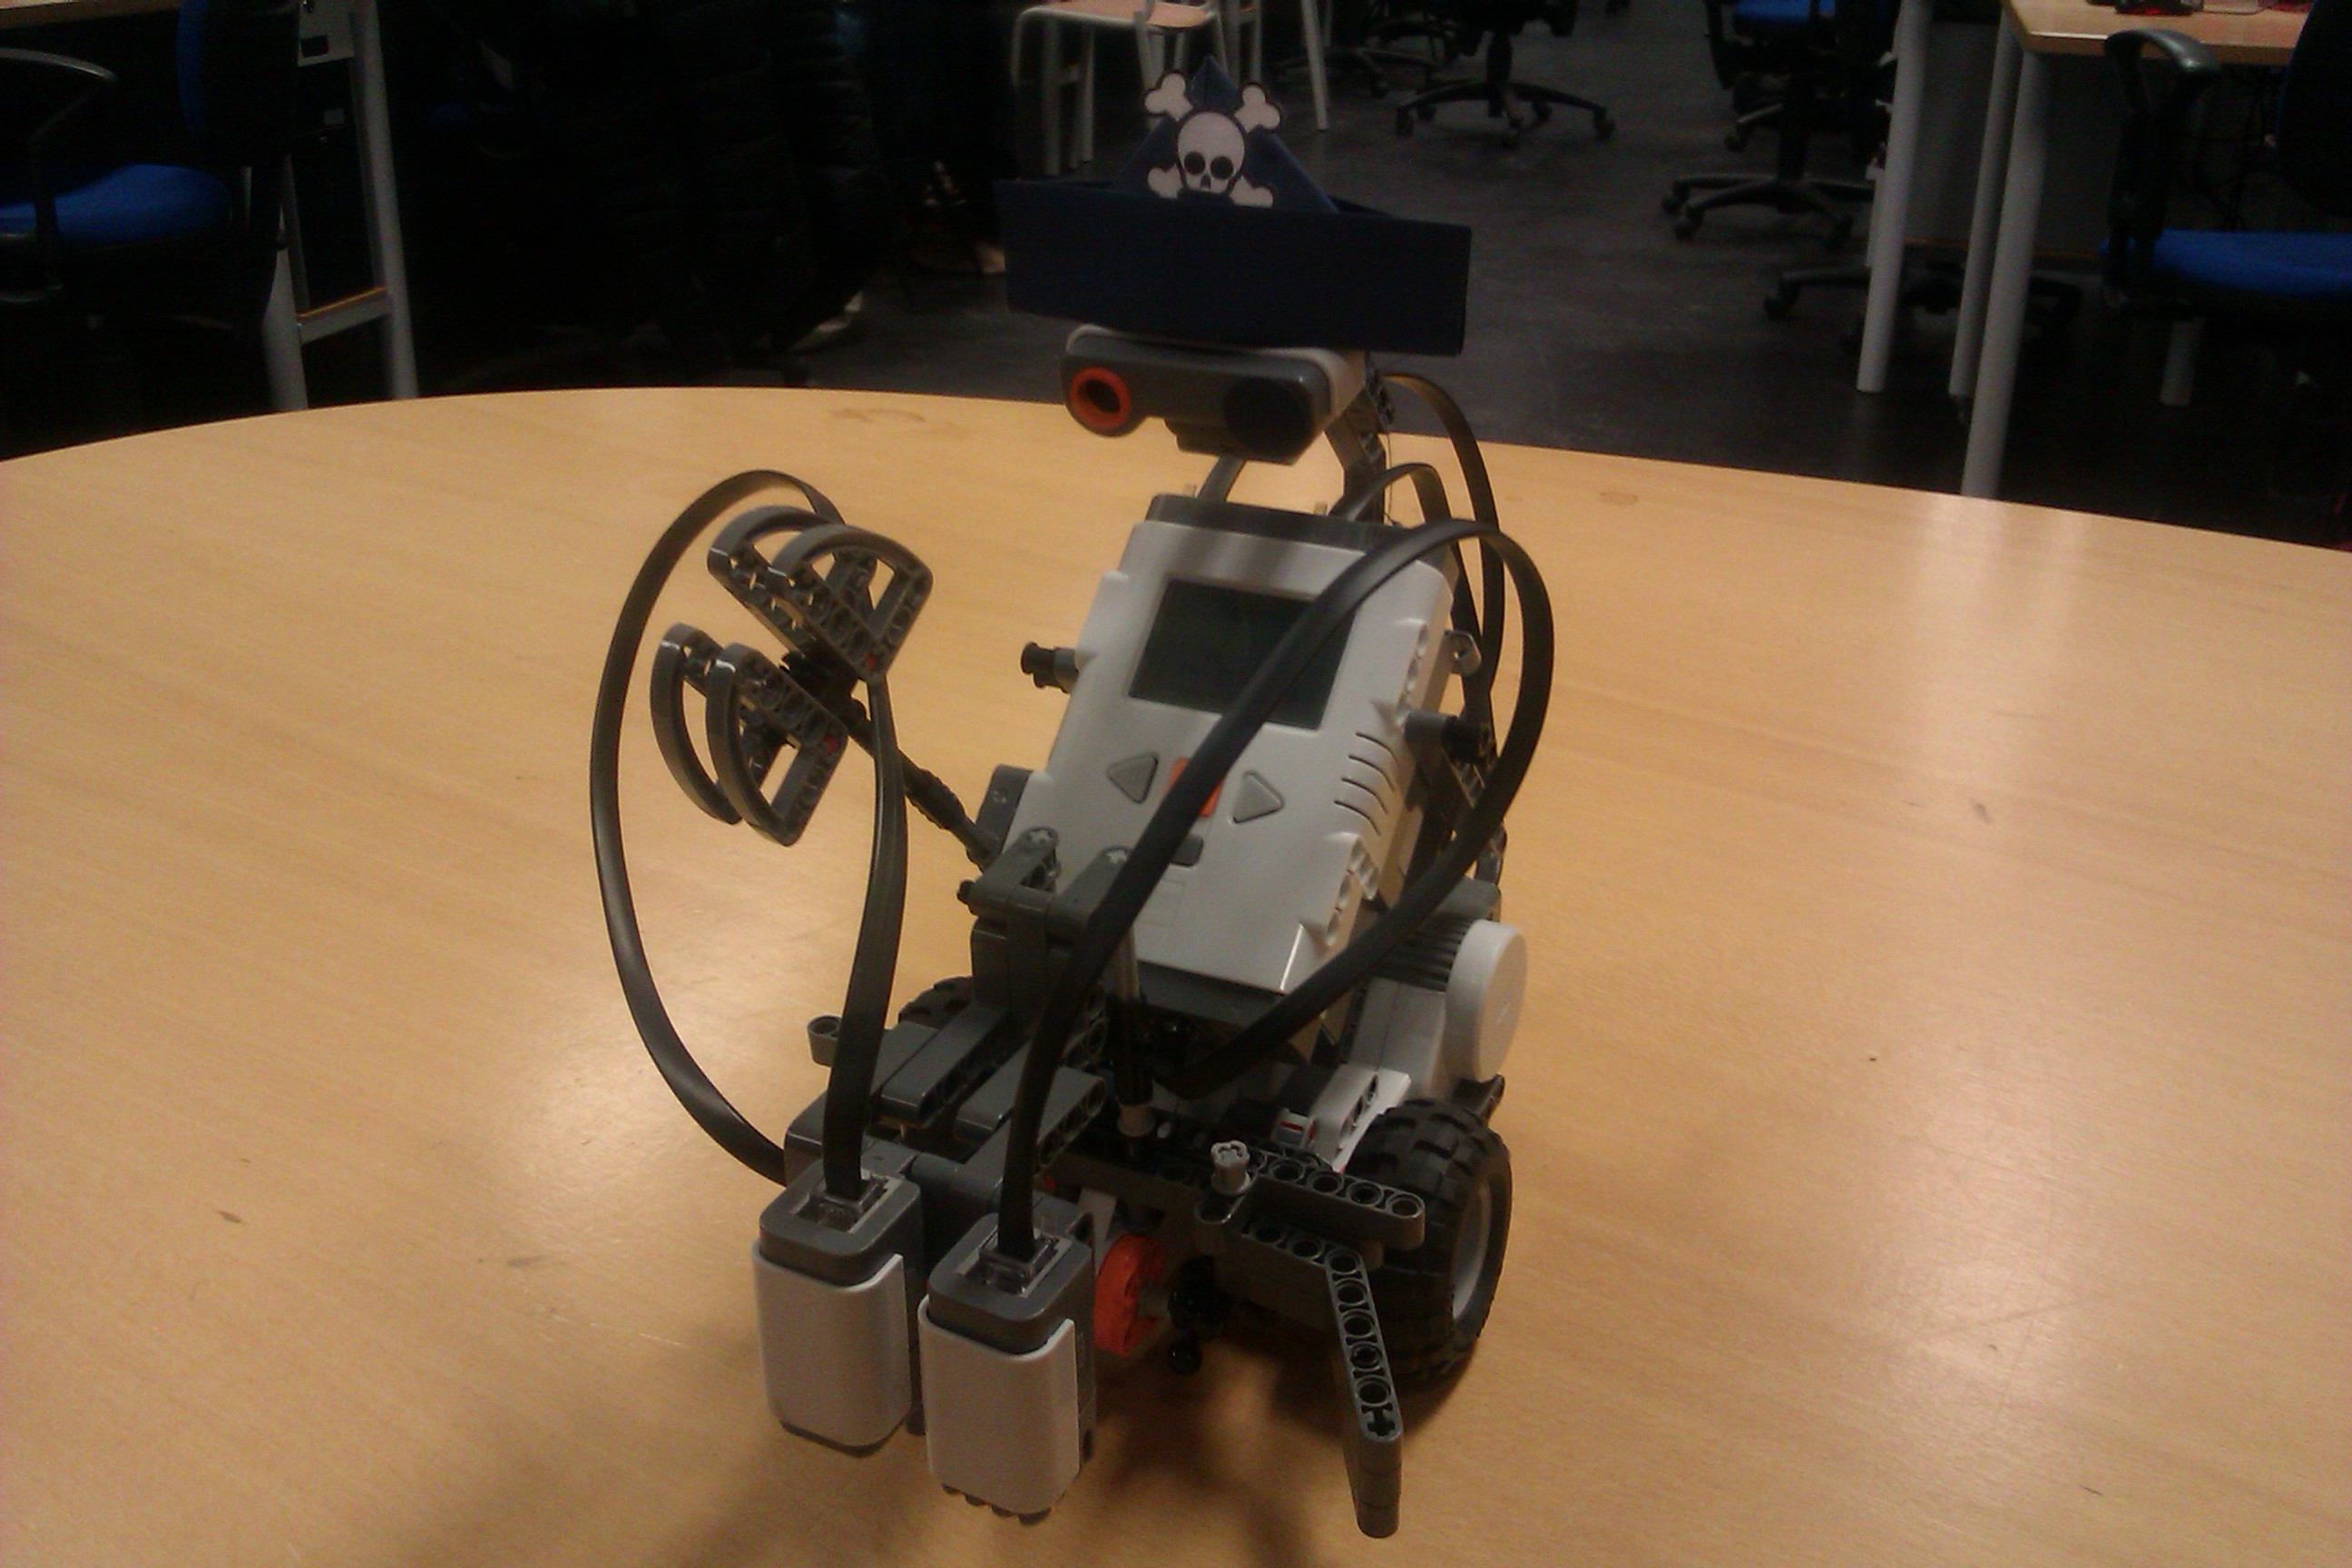
\includegraphics[width=0.5\textwidth]{images/pirate}
\end{figure}

\section*{Opdracht 2: stemgestuurde doolhof oplosser}
Het doel van de tweede opdracht is om je robot zo te programmeren dat hij "spraak-gestuurd" een doolhof op kan lossen. 
Helaas is het met deze NXT computers (ook wel bricks genoemd) erg moeilijk om spraakherkenning te maken. 
Voor deze opdracht zullen we ons dus beperken tot het horen van geluid om te bepalen of we links, rechts of rechtdoor moeten rijden. 

Op \url{http://bricxcc.sourceforge.net/nbc/nxcdoc/NXC_tutorial.pdf} kan je code vinden waarmee je je robot in kan programmeren. 
Uiteraard verwachten we niet dat je al kunt programmeren, daarom hebben we vast een deel van de code opgezet voor jullie. 
Deze code is te vinden op xxxxxxxxxxxxx.
Op sommige plekken in de voorbeeldcode staat: //Hier kan je code invoeren, het is de bedoeling dat je op deze plekken neerzet wat je robot moet doen. 
Omdat we er van uit gaan dat jullie nog niet heel goed kunnen programmeren zijn er een aantal functies gemaakt voor jullie die jullie kunnen gebruiken.
Deze functies zijn: \\
gaRechtdoor();\\
draaiNaarRechts();\\
draaiNaarLinks();\\
Zet deze codes neer op plekken waarvan het jullie slim lijkt. 
Uiteraard mogen jullie de door ons gemaakte code aanpassen!


\begin{figure}[h!]
	\caption{Een robot die bezig is met het oplossen van een doolhof}
	\centering
	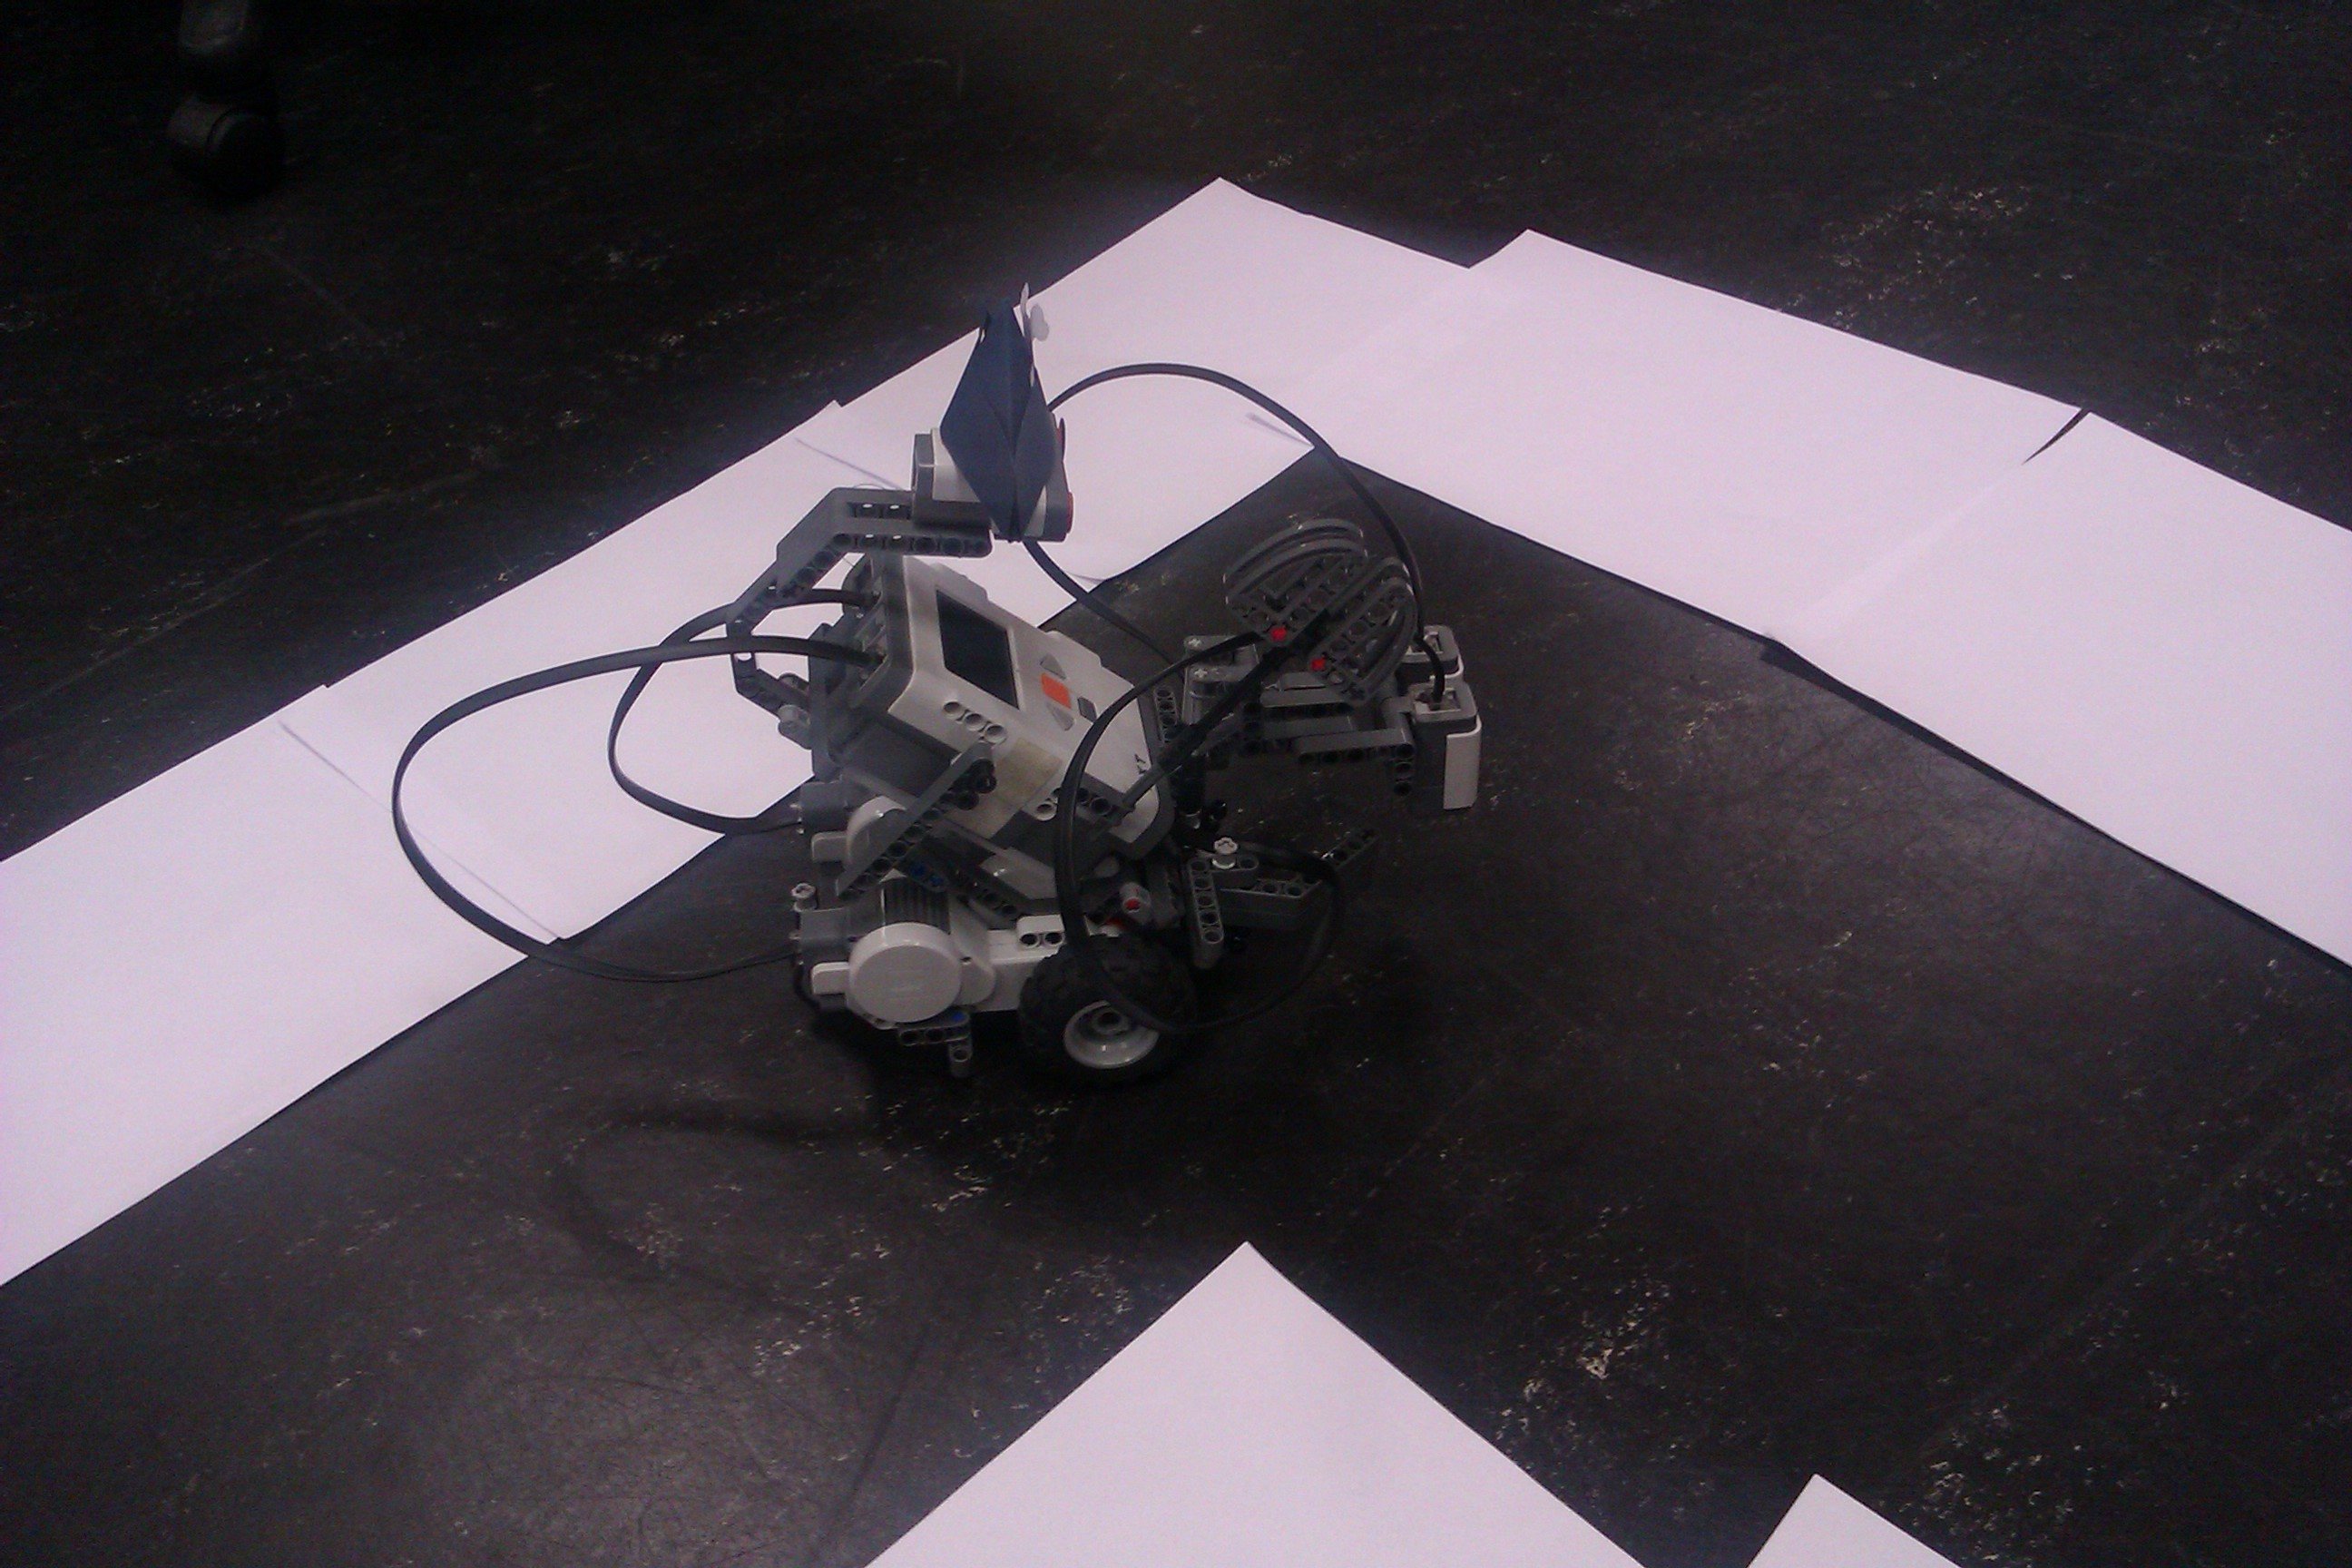
\includegraphics[width=0.5\textwidth]{images/maze}
\end{figure}
\section*{Opdracht 3: lijnvolger}
Het doel van de derde opdracht is het programmeren van een robot die een lijn kan volgen zonder externe input.
Deze autonome robot heeft als enige (zinnige) sensor de lichtsensor, omdat een zwarte ondergrond minder licht weerkaatst dan een witte ondergrond moet het volgen van een lijn hiermee mogelijk zijn. 
Wanneer je robot op de lijn zit hoeft je robot natuurlijk alleen maar rechtdoor te rijden, het wordt echter spannend wanneer de robot er van af is gereden. 
Zodra je robot van de lijn is gereden is natuurlijk de vraag of de lijn links zit, of dat de lijn toch iets meer naar rechts zit. 
Probeer ergens in je programma op te slaan hoever je naar links en naar rechts gaat kijken.
Nogmaals: wanneer je hulp nodig hebt kan je het altijd aan een van de begeleiders vragen!

\end{document}



